\documentclass[a4paper]{article}
\usepackage{geometry}
\usepackage{graphicx}
\usepackage[hidelinks]{hyperref}
\usepackage{times}
\usepackage{url}
\usepackage{fancyhdr}
\usepackage{titlesec}
\usepackage{xcolor}
\usepackage{listings} % Added for code formatting

\urlstyle{rm}

\setlength\parindent{0pt} % Removes all indentation from paragraphs

\geometry{
  top=1in,            % <-- you want to adjust this
  inner=1in,
  outer=1in,
  bottom=1in,
  headheight=3em,       % <-- and this
  headsep=2em,          % <-- and this
  footskip=3em,
}

\pagestyle{fancyplain}
\lhead{\fancyplain{}{Hwk 1 - Transforming a Table Into a Graph}}
\rhead{\fancyplain{}{BMI 881 - Scholarly Literature}}
\cfoot{\thepage}

\title{\textsc{BMI 881 - Hwk 1 - Transforming a Table Into a Graph}} % Title

\author{
Aurod Ounsinegad \\
}

\date{October $17^{th}$, 2024}

% Define Python code style
\lstdefinestyle{pythonstyle}{
    language=Python,
    basicstyle=\ttfamily\small,
    breaklines=true,
    keywordstyle=\color{blue},
    stringstyle=\color{green!50!black},
    commentstyle=\color{red!50!black},
    showstringspaces=false,
    numbers=left,
    numberstyle=\tiny,
    numbersep=5pt
}

\begin{document}

\maketitle

\section{Visualization of Mortality Rates}

Utilizing the Matplotlib library in Python, I produced a multi-panel line plot to display the mortality rate data from Feigin et al. (2014) Lancet 383:245-255. See the plot my code provided me below:

\begin{figure}[h!]
\centering
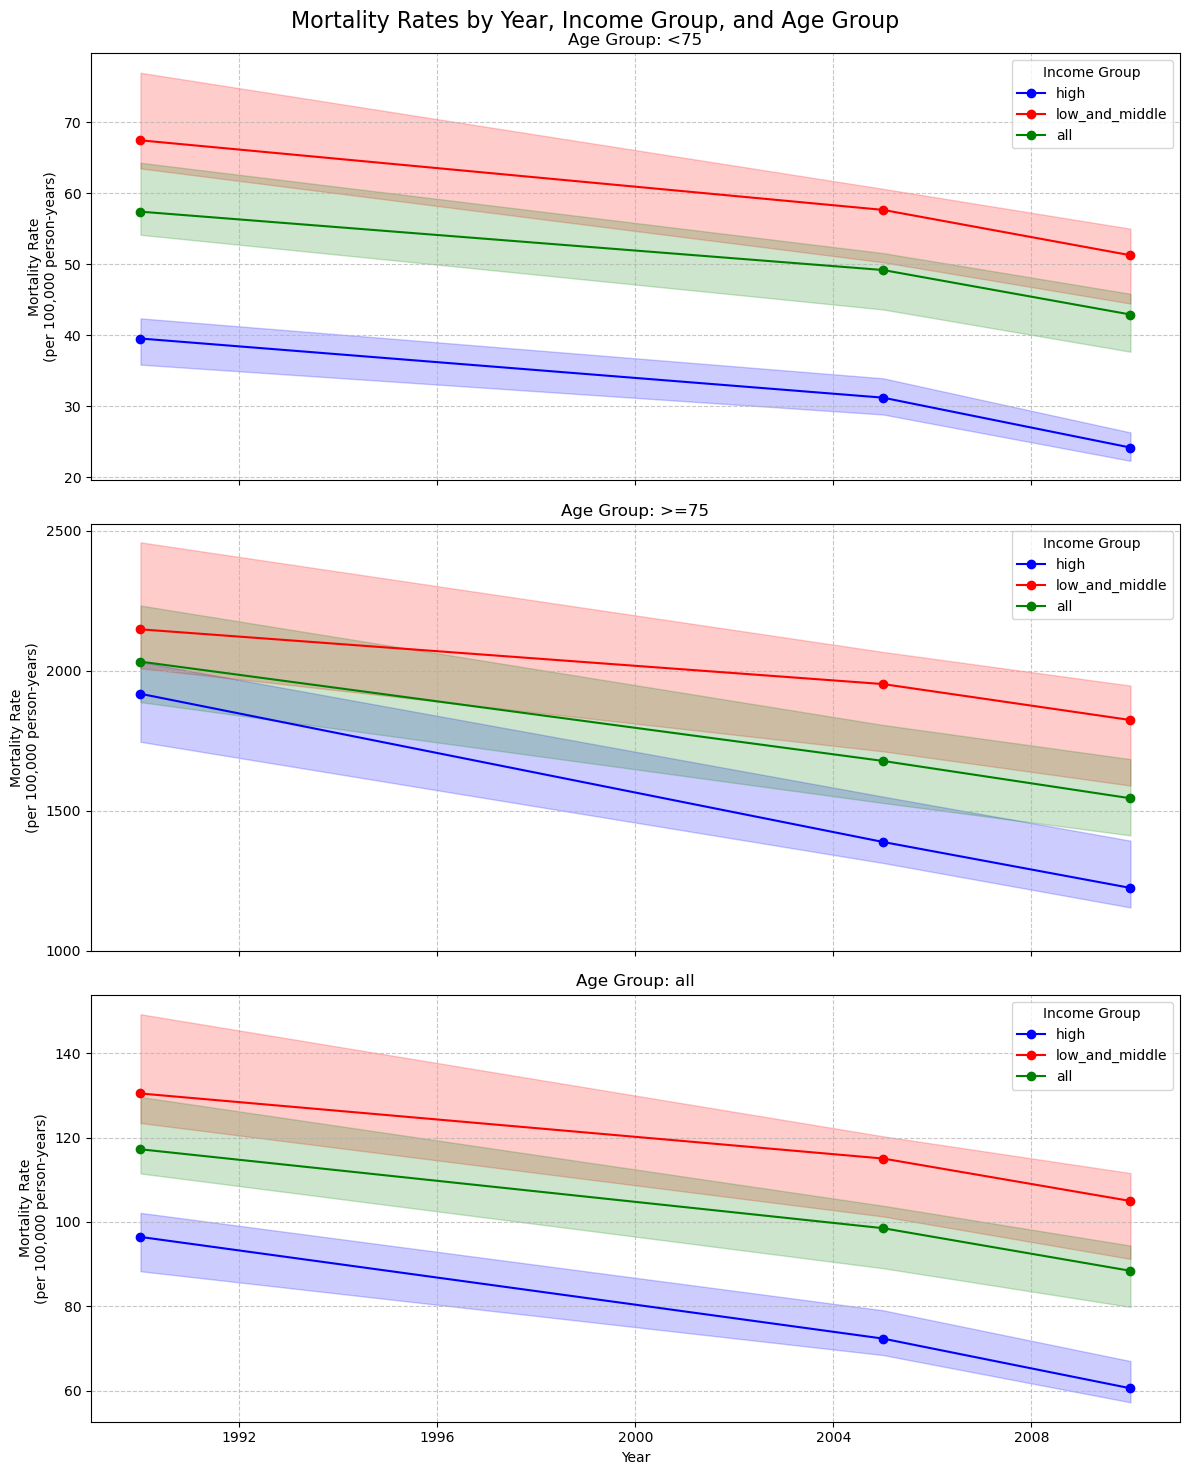
\includegraphics[width=0.85\textwidth]{HW1_table_to_graph_plot.png}
\caption{Mortality Rates by Year, Income Group, and Age Group}
\label{fig:mortality_rates}
\end{figure}

\section{Design Choices}

The design choices for this visualization were made to convey the intricate relationships between age groups, years, income groups, and mortality rates:

\begin{enumerate}
    \item \textbf{Multi-panel layout:} I utilized a 3x1 grid of subplots, with each subplot ($<$75, $\geq$75, all) indicating a distinct age group. As a result, comparisons within and between age groups can be made clearly and without scale problems.

    \item \textbf{Consistent color scheme:} High-income countries are shown in blue, low- and middle-income countries are shown in red, and the world average is shown in green. This uniformity facilitates visual comparison between panels.

    \item \textbf{Linear scale:} I first thought about using a logarithmic scale but ultimately decided to use a linear scale with unique y-axis ticks for every age group. This allows for clear trend representation and a more intuitive interpretation of the data.

    \item \textbf{Confidence intervals:} The 95\% confidence intervals are represented by the shaded areas surrounding each line, giving the data uncertainty a visual expression.

    \item \textbf{Clear labeling:} Each panel is labeled with its age group, and for ease of interpretation, the legend is the same on every panel.

    \item \textbf{Time series representation:} The x-axis represents years from 1990 to 2010, clearly showing trends over time.

    \item \textbf{Grid lines:} Light grid lines make it easier to read particular data and make comparisons between various income levels and years.

    \item \textbf{Custom y-axis scaling:} Custom y-axis scales for each panel that are suitable for the data range they represent enhance readability without sacrificing the ability to compare trends.
\end{enumerate}

These design choices produce a thorough and simple-to-understand representation that conveys the intricacy of the data effectively and permits many degrees of comparison.

\section{Comprehensive Graph Concept}

Below are my suggestions on how you could combine all the data from the original table into a single, comprehensive graph:

\begin{enumerate}
    \item \textbf{Base structure:} Keep the current multi-panel arrangement as it allows for easy comparison and efficiently divides age groups.

    \item \textbf{Additional metrics:} Add other graphical components, such as bar charts overlaid on the current lines, or use supplementary y-axes to incorporate additional metrics, such as incidence, prevalence, etc.

    \item \textbf{Interactive elements:} Implement interactivity using tools like Plotly or Bokeh, allowing users to:
    \begin{itemize}
        \item Toggle between different metrics
        \item Zoom in on specific time periods or data ranges
        \item Hover over data points to see exact values and additional information
    \end{itemize}

    \item \textbf{Annotations:} Add text annotations to highlight key findings or significant changes in trends.

    \item \textbf{Color coding:} Use a consistent color scheme across all metrics to represent income groups, enhancing comparability.

    \item \textbf{Layered information:} Develop a system that allows users to gradually add layers of data, beginning with the fundamental trends in mortality rates and progressing to increasingly intricate comparisons between indicators.
\end{enumerate}

With the above method, all the data from the original table would be captured in a rich, interactive display that would still be understandable and easy to use. Users would be able to examine the data at different degrees of detail thanks to the interactivity, which makes it appropriate for both a brief summary and a thorough examination.

\appendix
\section{Python Code}

The following Python code was used to generate the visualization:

\lstinputlisting[style=pythonstyle]{HW1_table_to_graph.py}

\end{document}
